%% Copyright (C) 2010, Gostai S.A.S.
%%
%% This software is provided "as is" without warranty of any kind,
%% either expressed or implied, including but not limited to the
%% implied warranties of fitness for a particular purpose.
%%
%% See the LICENSE file for more information.
\chapter{Urbi for ROS Users}
\setHtmlFileName{ros-tutorial}
\label{sec:tut:ros}


This chapter extends the ROS official tutorials
(\url{http://www.ros.org/wiki/ROS/Tutorials}).  Be sure to complete this
tutorial before reading this document.

\section{Communication on topics}

First we will take back examples about topics; make sure that talker and
listener in the \file{beginner\_tutorial} package are compiled. You can
recompile it with the following command:

\begin{shell}
$ rosmake beginner_tutorial
\end{shell}

\subsection{Starting a process from Urbi}

To communicate with ROS components, you need to launch them. You can do it
by hand, or ask \urbi to do it for you. To launch new processes through
\urbi, we will use the class \refObject{Process}.

Let's say we want to start \command{roscore}, and the talker of the beginner
tutorial.  Open an \urbi shell by typing the command \samp{rlwrap urbi
  -i}.  Here \command{rlwrap} makes \samp{urbi -i} acts like a shell prompt,
with features like line editing, history, \ldots

\begin{urbiunchecked}
var core = Process.new("roscore", []);
[00000001] Process roscore
var talker = Process.new("rosrun", ["beginner_tutorial", "talker"]);
[00000002] Process rosrun
core.run;
talker.run;
\end{urbiunchecked}

At this point, the processes are launched. The first argument of
\lstinline{Process.new} is the name of the command to launch, the second is
a list of arguments.

Then you can check the status of the processes, get their stdout/stderr
buffers, kill them in \us (see \refObject{Process}).


\subsection{Listening to Topics}

First you need to make sure that \command{roscore} is running, and the Ros
module is loaded correctly:

\begin{urbiunchecked}
Global.hasLocalSlot("Ros");
[00016931] true
\end{urbiunchecked}

\noindent
Then we can get the list of launched nodes:

\begin{urbiunchecked}
Ros.nodes;
\end{urbiunchecked}

This returns a \refObject{Dictionary} with the name of the node as key, and
a dictionary with topics subscribed, topics advertised, topics advertised as
value.

We can check that our talker is registered, and on which channel it
advertises:

\begin{urbiunchecked}
// Get the structure.
// "|;" is an idiom to discard the display of the return value.
var nodes = Ros.nodes|;

// List of nodes (keys).
nodes.keys;
[00000002] ["/rosout", "/urbi_1273060422295250703", "/talker"]

// Details of the node "talker".
nodes["talker"]["publish"];
[00000003] ["/rosout", "/chatter"]
\end{urbiunchecked}

Here we see that this node advertises \file{/rosout} and
\file{/chatter}. Let's subscribe to \file{/chatter}:

\begin{urbiunchecked}
// Initialize the subscription object.
var chatter = Ros.Topic.new("/chatter")|;
// Subscribe.
chatter.subscribe;
// This is the way we are called on new message.
var chatTag = Tag.new|;
chatTag: at (chatter.onMessage?(var e))
  // This will be executed on each message.
  echo(e);
\end{urbiunchecked}

In this code, \lstinline{e} is a Dictionary that follows the structure of
the ROS message. Here is an example of what this code produces:

\begin{urbiunchecked}
[00000004] *** ["data" => "Hello there! This is message [4]"]
[00000005] *** ["data" => "Hello there! This is message [5]"]
[00000006] *** ["data" => "Hello there! This is message [6]"]
\end{urbiunchecked}

We can also get a template for the message structure on this channel with:

\begin{urbiunchecked}
chatter.structure;
[00000007] ["data" => ""]
\end{urbiunchecked}

To stop temporarily the \refSlot[Global]{echo}, we take advantages of tags
(\autoref{sec:tut:tags}), by doing \lstinline{chatTag.freeze}.  Same thing
goes with unfreeze.  Of course you could also call
\lstinline{chatter.unsubscribe}, which unsubscribes you completely from this
channel.


\subsection{Advertising on Topics}

To advertise a topic, this is roughly the same procedure.


\subsubsection{Simple Talker}

Here is a quick example:

\begin{urbiunchecked}
// Initialize our object.
var talker = Ros.Topic.new("/chatter")|;
// Advertise (providing the ROS Type of this topic).
talker.advertise("std_msgs/String");

// Get a template of our structure.
var msg = talker.structure.new;
msg["data"] = "Hello ROS world"|;
talker << msg;
\end{urbiunchecked}

We have just sent our first message to ROS, here if you launch the chatter,
you will be able to get the message we have just sent.

The \lstinline{<<} operator is an convenient alias for
\refSlot[Ros.Topic]{publish}.



\subsubsection{Turtle Simulation}
\label{sec:turtlesim}

Now we are going to move the turtle with \urbi. First let's launch the
turtle node:

\begin{urbiunchecked}
var turtle = Process.new("rosrun", ["turtlesim", "turtlesim_node"])|;
turtle.run;
\end{urbiunchecked}

With the help of \refSlot[Ros]{topics}, we can see that this turtle
subscribes to a topic \file{/turtle1/command\_velocity}. Let's advertise on
it:

\begin{urbiunchecked}
var velocity = Ros.Topic.new("/turtle1/command_velocity")|;
velocity.advertise("turtlesim/Velocity");
velocity.structure;
[00000001] ["linear" => 0, "angular" => 0]
\end{urbiunchecked}


Now we want to have it moving in circle with a small sinusoid wave.  This
goes in two step.  First, we set up the infrastructure so that changes in
\urbi are seamlessly published in ROS.

\begin{urbiunchecked}
// Get our template structure.
var m = velocity.structure.new |;
m["linear"] = 0.8 |;
var angular = 0 |;
// Every time angular is changed, we send a message.
at (angular->changed?)
{
  m["angular"] = angular;
  velocity << m
};
\end{urbiunchecked}

\noindent
In the future \urbi will provide helping functions to spare the user from
the need to perform this ``binding''.  But once this is done, all the
features of \us can be used transparently.  For instance we can assign a
sinusoidal trajectory to \samp{angular}, which results in the screen-shot on
the right-hand side.

\begin{multicols}{2}
\begin{urbiunchecked}
// A Tag to control the following endless
// statement.
var angTag = Tag.new|;

angTag:
  // Bind "angular" to a trajectory.
  // Put in background thanks to ",",
  // since this statement is never ending.
  angular = 0.3 sin: 2s ampli: 2,

// Leave 20 seconds to the turtle...
sleep(20s);

// before freezing it.
angTag.freeze;
\end{urbiunchecked}

\columnbreak

\begin{center}
  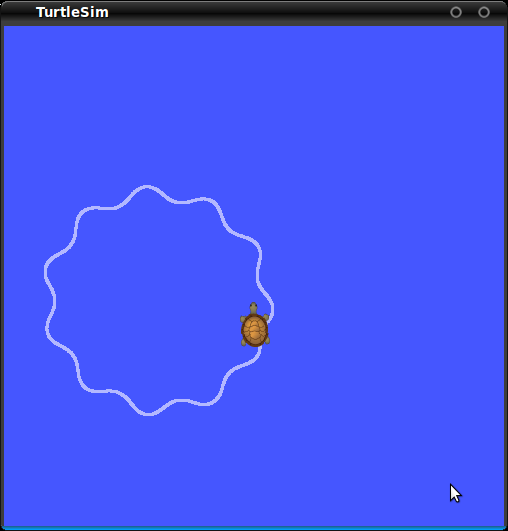
\includegraphics[width=0.45\textwidth]{img/turtlesim-tutorial}
\end{center}

\end{multicols}

We won't cover this code in details, but the general principle is that
\lstinline{angular} is updated every 20ms with the values of a sinusoid wave
trajectory with 0.3 as average value, 2 seconds for the period and 2 for the
amplitude.  See \refObject{TrajectoryGenerator} for more information.

Every time \lstinline{angular} is changed, a new message is sent on the
Topic \file{/turtle1/command\_velocity}, thus updating the position of the
turtle.  After 20 seconds the tag is frozen, pausing the trajectory
generation and the \lstinline{at}.

\section{Using Services}

Services work the same way topics do, with minor differences.

Let's take back the turtle simulation example (\autoref{sec:turtlesim}).
Then we can list the available services, and filter out loggers:

\begin{urbiunchecked}
var logger = Regexp.new("(get|set)_logger") |;
var services = Ros.services.keys |;
services.filter(closure (var item) { item not in logger });
[00000001] ["/clear", "/kill", "/turtle1/teleport_absolute", "/turtle1/teleport_relative", "/turtle1/set_pen", "/reset", "/spawn"]
\end{urbiunchecked}

The \lstinline{closure} construct allows us to keep access to the local
variables, here \lstinline{logger}.

Now there is a service called \file{/spawn}; to initialize it:

\begin{urbiunchecked}
var spawn = Ros.Service.new("/spawn", false) |;
waituntil(spawn.initialized);
\end{urbiunchecked}

The \lstinline{new} function takes the service name as first argument, and
whether or not the connection should be kept alive as second argument.

Since the creation of this object checks the service name, you should wait
until \lstinline{initialized} is true to use this service.  You can also see
the structure of the request through \lstinline{spawn.reqStruct}, and the
structure of the response by doing \lstinline{spawn.resStruct}.

Now let's spawn a turtle called Jenny, at position (4, 4).

\begin{urbiunchecked}
var req = spawn.reqStruct.new |;
req["x"] = 4 |
req["y"] = 4 |
req["name"] = "Jenny" |;
spawn.request(req);
[00000001] ["name" => "Jenny"]
\end{urbiunchecked}

\bigskip

Now, if you want to go further, please see the reference manual section
about ROS, \autoref{sec:specs:ros}.

%%% Local Variables:
%%% mode: latex
%%% TeX-master: "../urbi-sdk"
%%% ispell-dictionary: "american"
%%% ispell-personal-dictionary: "../urbi.dict"
%%% fill-column: 76
%%% End:
